% 4,6 : Paul
% 7,8 : Jo'
% 9,10,11,13: Anthony

\documentclass{article}

\usepackage{a4}
\usepackage{amsmath}
\usepackage{amsfonts}
\usepackage{amssymb}
\usepackage{float}
\usepackage[utf8]{inputenc}
\usepackage[T1]{fontenc}

\usepackage{framed}

\usepackage{graphicx}
\usepackage{caption}
\usepackage{subcaption}
\usepackage{wrapfig}

\usepackage{geometry}


\usepackage{fullpage,graphicx}
\usepackage{rotating}

\usepackage{multirow}

%\setlength{\hoffset}{-18pt}
\setlength{\oddsidemargin}{0cm}     % Marge gauche sur pages impaires
\setlength{\evensidemargin}{0cm}    % Marge gauche sur pages paires
\setlength{\marginparwidth}{54pt}   % Largeur de note dans la marge
\setlength{\textwidth}{17cm}       % Largeur de la zone de texte (17cm)
\setlength{\marginparsep}{7pt}      % Séparation de la marge
\setlength{\topmargin}{-1cm}         % Pas de marge en haut
\setlength{\headheight}{0cm}       % Haut de page
\setlength{\headsep}{10pt}          % Entre le haut de page et le texte
\setlength{\footskip}{27pt}         % Bas de page + séparation
\setlength{\textheight}{23cm}      % Hauteur de la zone de texte (25cm)

\setlength{\parskip}{1ex}
\setlength{\parindent}{1cm}

%\setlength{\topsep}{500pt}
\setlength{\abovecaptionskip}{0.1cm}
\setlength{\belowcaptionskip}{0.5cm}



\newlength{\leftbarwidth}
\setlength{\leftbarwidth}{3pt}
\newlength{\leftbarsep}
\setlength{\leftbarsep}{10pt}
\newlength{\leftbarmargin}
\setlength{\leftbarmargin}{0pt}
\newlength{\defaultparindent}
\setlength{\defaultparindent}{\parindent}


\renewenvironment{leftbar}{%
    \def\FrameCommand{\hspace{\leftbarmargin} \vrule width \leftbarwidth \relax\hspace{\leftbarsep}}%
    \MakeFramed {\advance \hsize -\width \FrameRestore }%
}{%
    \endMakeFramed
}


%\newenvironment{defx}{\noindent \\ \textbf{Definition:} \vspace{-11pt} \begin{leftbar} \vspace{4pt}}{\end{leftbar}}
%\newenvironment{propx}{\noindent \\ \textbf{Proposition:} \vspace{-11pt} \begin{framed}}{\end{framed}}

\newenvironment{defx}{
\setlength{\leftbarwidth}{3pt} 
\setlength{\leftbarmargin}{-2pt} 
\setlength{\leftbarsep}{10pt} 
\begin{leftbar}}{\end{leftbar}}
\newenvironment{propx}{\begin{framed}}{\end{framed}}

\newenvironment{demox}{\footnotesize \noindent \textit{Demo:}  \vspace{-9pt} 
\setlength{\leftbarwidth}{1pt} 
\setlength{\leftbarmargin}{5pt}
\setlength{\leftbarsep}{3pt} 
\setlength{\parindent}{7pt}

\begin{leftbar}}{\end{leftbar}
\setlength{\parindent}{\defaultparindent}
\normalsize}



\newenvironment{deft}[1]{\noindent \\ \textbf{\textsc{#1}} \vspace{-11pt} \setlength{\leftbarwidth}{3pt} 
\setlength{\leftbarmargin}{-2pt} 
\setlength{\leftbarsep}{10pt} 
\begin{leftbar} \vspace{4pt}}{\end{leftbar}}
\newenvironment{propt}[1]{\noindent \\ \textbf{\textsc{#1}} \vspace{-11pt} \begin{framed}}{ \end{framed}}


\newenvironment{algot}[1]{\noindent \\ \textbf{\textsc{#1}} \par \nobreak \vspace{1pt}\hrule\vspace{0pt} \setlength{\parindent}{0cm} \ttfamily} {\normalfont \setlength{\parindent}{\defaultparindent} \par \nobreak \vspace{4pt}\hrule\vspace{15pt}}

\newenvironment{algox}{\noindent \\  \par \nobreak \vspace{1pt}\hrule\vspace{0pt} \setlength{\parindent}{0cm} \ttfamily} {\normalfont \setlength{\parindent}{\defaultparindent} \par \nobreak \vspace{4pt}\hrule\vspace{15pt}}

%\newenvironment{algot}[1]{\noindent \\ \textbf{\textsc{#1}} \par \nobreak \vspace{1pt}\hrule\vspace{0pt} \setlength{\parindent}{0cm} \ttfamily \begin{tabbing} ~~~~\=~~~~\=~~~~\=~~~~\=~~~~\=~~~~\=~~~~} {\end{tabbing} \normalfont \setlength{\parindent}{\defaultparindent} \par \nobreak \vspace{4pt}\hrule \\}

\newcommand{\comment}[1]{\hfill// #1}

\newcommand{\bbB}{\mathbb{B}}
\newcommand{\bbN}{\mathbb{N}}
\newcommand{\bbZ}{\mathbb{Z}}
\newcommand{\bbR}{\mathbb{R}}

\newcommand{\tb}{.~~~~}

%\newcommand{\exsubpart}[1]{\subsection*{#1)}\\ }
\newcommand{\exsubpart}[1]{\subsection*{#1)} \vspace{-51pt} ~\\}

\newcommand{\info}[1]{\small{\textit{(#1)}}}



\graphicspath{{./Images/}}

\begin{document}

\noindent {\fontsize{20}{20}\selectfont \noindent \textbf{Laboratoire d'électronique~:}}

\noindent {\fontsize{30}{30}\selectfont \noindent \textbf{Convertisseurs A/N et N/A}}

\vspace{5pt}\hrule\vspace{2pt}

\noindent {\Large \textbf{\textsc{Masur} Jonathan}\hfill\textbf{\textsc{Graignic} Anthony}\hfill \textbf{\textsc{Gosselin} Paul}}

\vspace{20pt}


% Return loss

% 4.2.2
% Désadaptation d'impédance
% Voir HF-VHF : 2.16, 3.22





\section{L'amplificateur accordé}

\subsection{Description}

On considère l'amplificateur accordé décrit Fig.~\ref{schem6}.

\begin{figure}[h!]
	\centering
	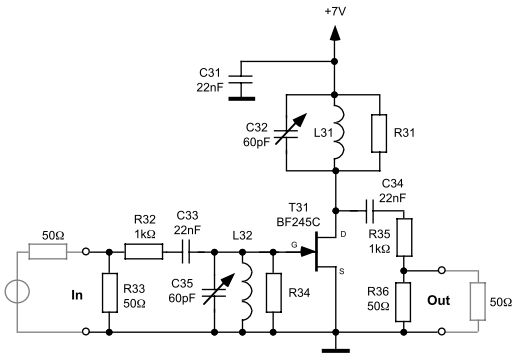
\includegraphics[width=.7\textwidth]{schem6}
	\caption{}
	\label{schem6}
\end{figure}


\subsection{Questions et calculs}

\exsubpart{1}

Les deux circuits résonnants sont couplés via un couplage actif.

\exsubpart{2}

On couple deux filtres d'ordre 1, formant ainsi un filtre d'ordre 2.

Si le facteur de qualité de chacun des circuits résonants est le même, on obtient donc un facteur de qualité global de~:
\begin{equation*}
Q_{tot} = \frac{1}{\sqrt{2^{1/2}-1}}Q = 1,554 Q
\end{equation*}


\exsubpart{3}

Les condensateurs $C_{33}$ et $C_{34}$ permettent uniquement de couper de très basses fréquences, hors de notre domaine d'intérêt. On peut donc les ignorer.

Les filtres restants en amont et en aval du JFET sont tout deux constitués d'une inductance et d'une capacité en parallèle, liées à une tension de référence. Ce sont deux passe-bande d'ordre 2~: l'ordre est de 1 de chaque côté de la fréquence de résonance, donnant donc lieu à des pentes de $\pm$20 dB/décade de part et d'autre de cette fréquence.

En couplant ces deux filtres, on obtient donc un filtre passe-bande d'ordre total 4. On trouve de part et d'autre de la fréquence de résonance $f_0$ un ordre 2, soit des pentes de +20 dB/décade et -20 dB/décade respectivement en-dessous et au-dessus de $f_0$.


\exsubpart{4}

Afin d'obtenir une bande passante à -3dB s'étendant de $f_1 = $13 MHz à $f_2 = $15 MHz, le facteur de qualité total doit être de~:
\begin{equation*}
Q_{tot} = \frac{f_0}{f_2-f_1}
\end{equation*}
avec $f_0 = $14 MHz, soit~:
\begin{equation*}
Q_{tot} = 7
\end{equation*}

Cela correspond pour chaque circuit résonant à un facteur de qualité de~:
\begin{equation*}
Q = \sqrt{2^{1/2}-1}~Q_{tot} = 4,505
\end{equation*}


%Toutefois, on prendra $R_{31}=R_{34}=\infty$~: en effet, ces résistances on juste pour but de diminuer les facteurs de qualité des filtres situés en amont et en aval du JFET.
% L31 = L32 = 2.2 uH


% 5) On saute...





\section{L'oscillateur à quartz}

\subsection{Description}

%TODO

\subsection{Question et calculs}

\section{Mélangeurs}

\subsection{Introduction}
Les mélangeurs sont des circuits qui permettent de multiplier deux signaux sinusoïdaux.
D'après la formule d'addition des sinus :
\begin{center}
$\sin(\omega_{1}\cdot t)\cdot \sin(\omega_{2}\cdot t) = \frac{1}{2}\cdot(\cos((\omega_{1} - \omega_{2})\cdot t) - cos((\omega_{1} + \omega_{2})\cdot t ) )$
\end{center}

Pour un montage idéal, nous avons donc une première composante fréquentielle en $\omega_{1} - \omega_{2}$ et une deuxième en $\omega_{1} + \omega_{2}$

Il est alors possible par filtrage d'éliminer l'une de ces deux composantes, typiquement $\omega_{1} - \omega_{2}$, afin de ne garder que la composante en $\omega_{1} + \omega_{2}$.\\

Ceci est utile pour réaliser plusieurs types de modulation et de démodulation.
\\
En pratique, la multiplication va présenter des non linéarités, nous aurons donc des harmoniques de $\omega_{1}$ et de $\omega_{2}$ en entrée du système.
Ainsi, nous avons des composantes à toutes les fréquences : $m \cdot \omega_{1} + n \cdot \omega_{2}$, $\forall m, n \in\bbZ$


\subsubsection{Mélangeur à cellule de Gilbert}q

La multiplication des signaux IN1 et IN2 est faite par le circuit intégré NE602. 
Il s'agit d'un multiplicateur à 4 quadrants, c'est à dire que la sortie est valable pour toutes les combinaisons possibles des signes des tensions IN1 et IN2 (+, +), (+, -), (-, +) et (-, -).
Il n'y a donc aucunement besoin de polariser les entrées avec une composante continue, d'où un montage très simple.\\

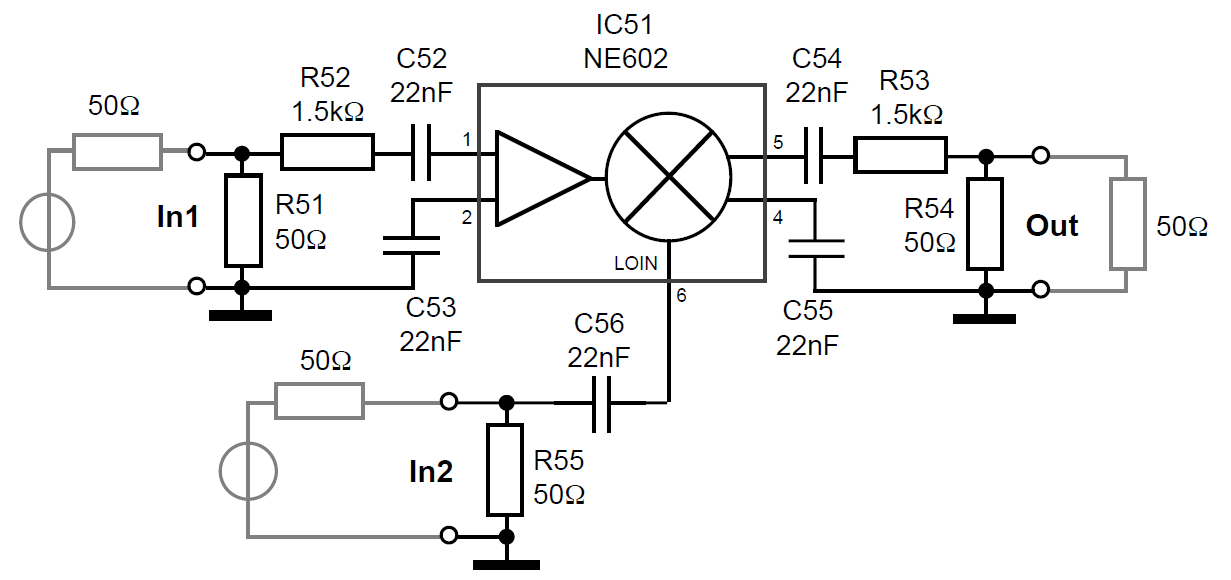
\includegraphics{shema_melangeur_gilbert.png}

L'impédence d'entrée sur l'amplificateur différentiel (broches 1 et 2) est d'environ $1.5k\Omega$ \footnote{Voir datasheet du composant NE602}. Idem pour les sorties sur les broches 4 et 5.
Les résistances R51, R52, R53 et R54 servent à adapter l'impédance du câble d'antenne $50\Omega$ vers le circuit intégré.\\

Le circuit à été prévu pour fabriquer un oscillateur avec les broches 6 et 7 cependant on n'utilise pas cette fonctionnalité, car nous avons notre propre oscillateur. L'amplitude doit être au moins de $200mV$ pour simuler un oscillateur local, contrairement à l'entrée des broches 1 et 2 qui simule une antenne.
En effet par la conception même le circuit n'est pas complètement symétrique, il serait possible d'inverser les deux entrées mais les amplitudes ne correspondraient pas à un fonctionnement optimal du circuit. % A étudier - clarifier
\\
Spectre de sortie :
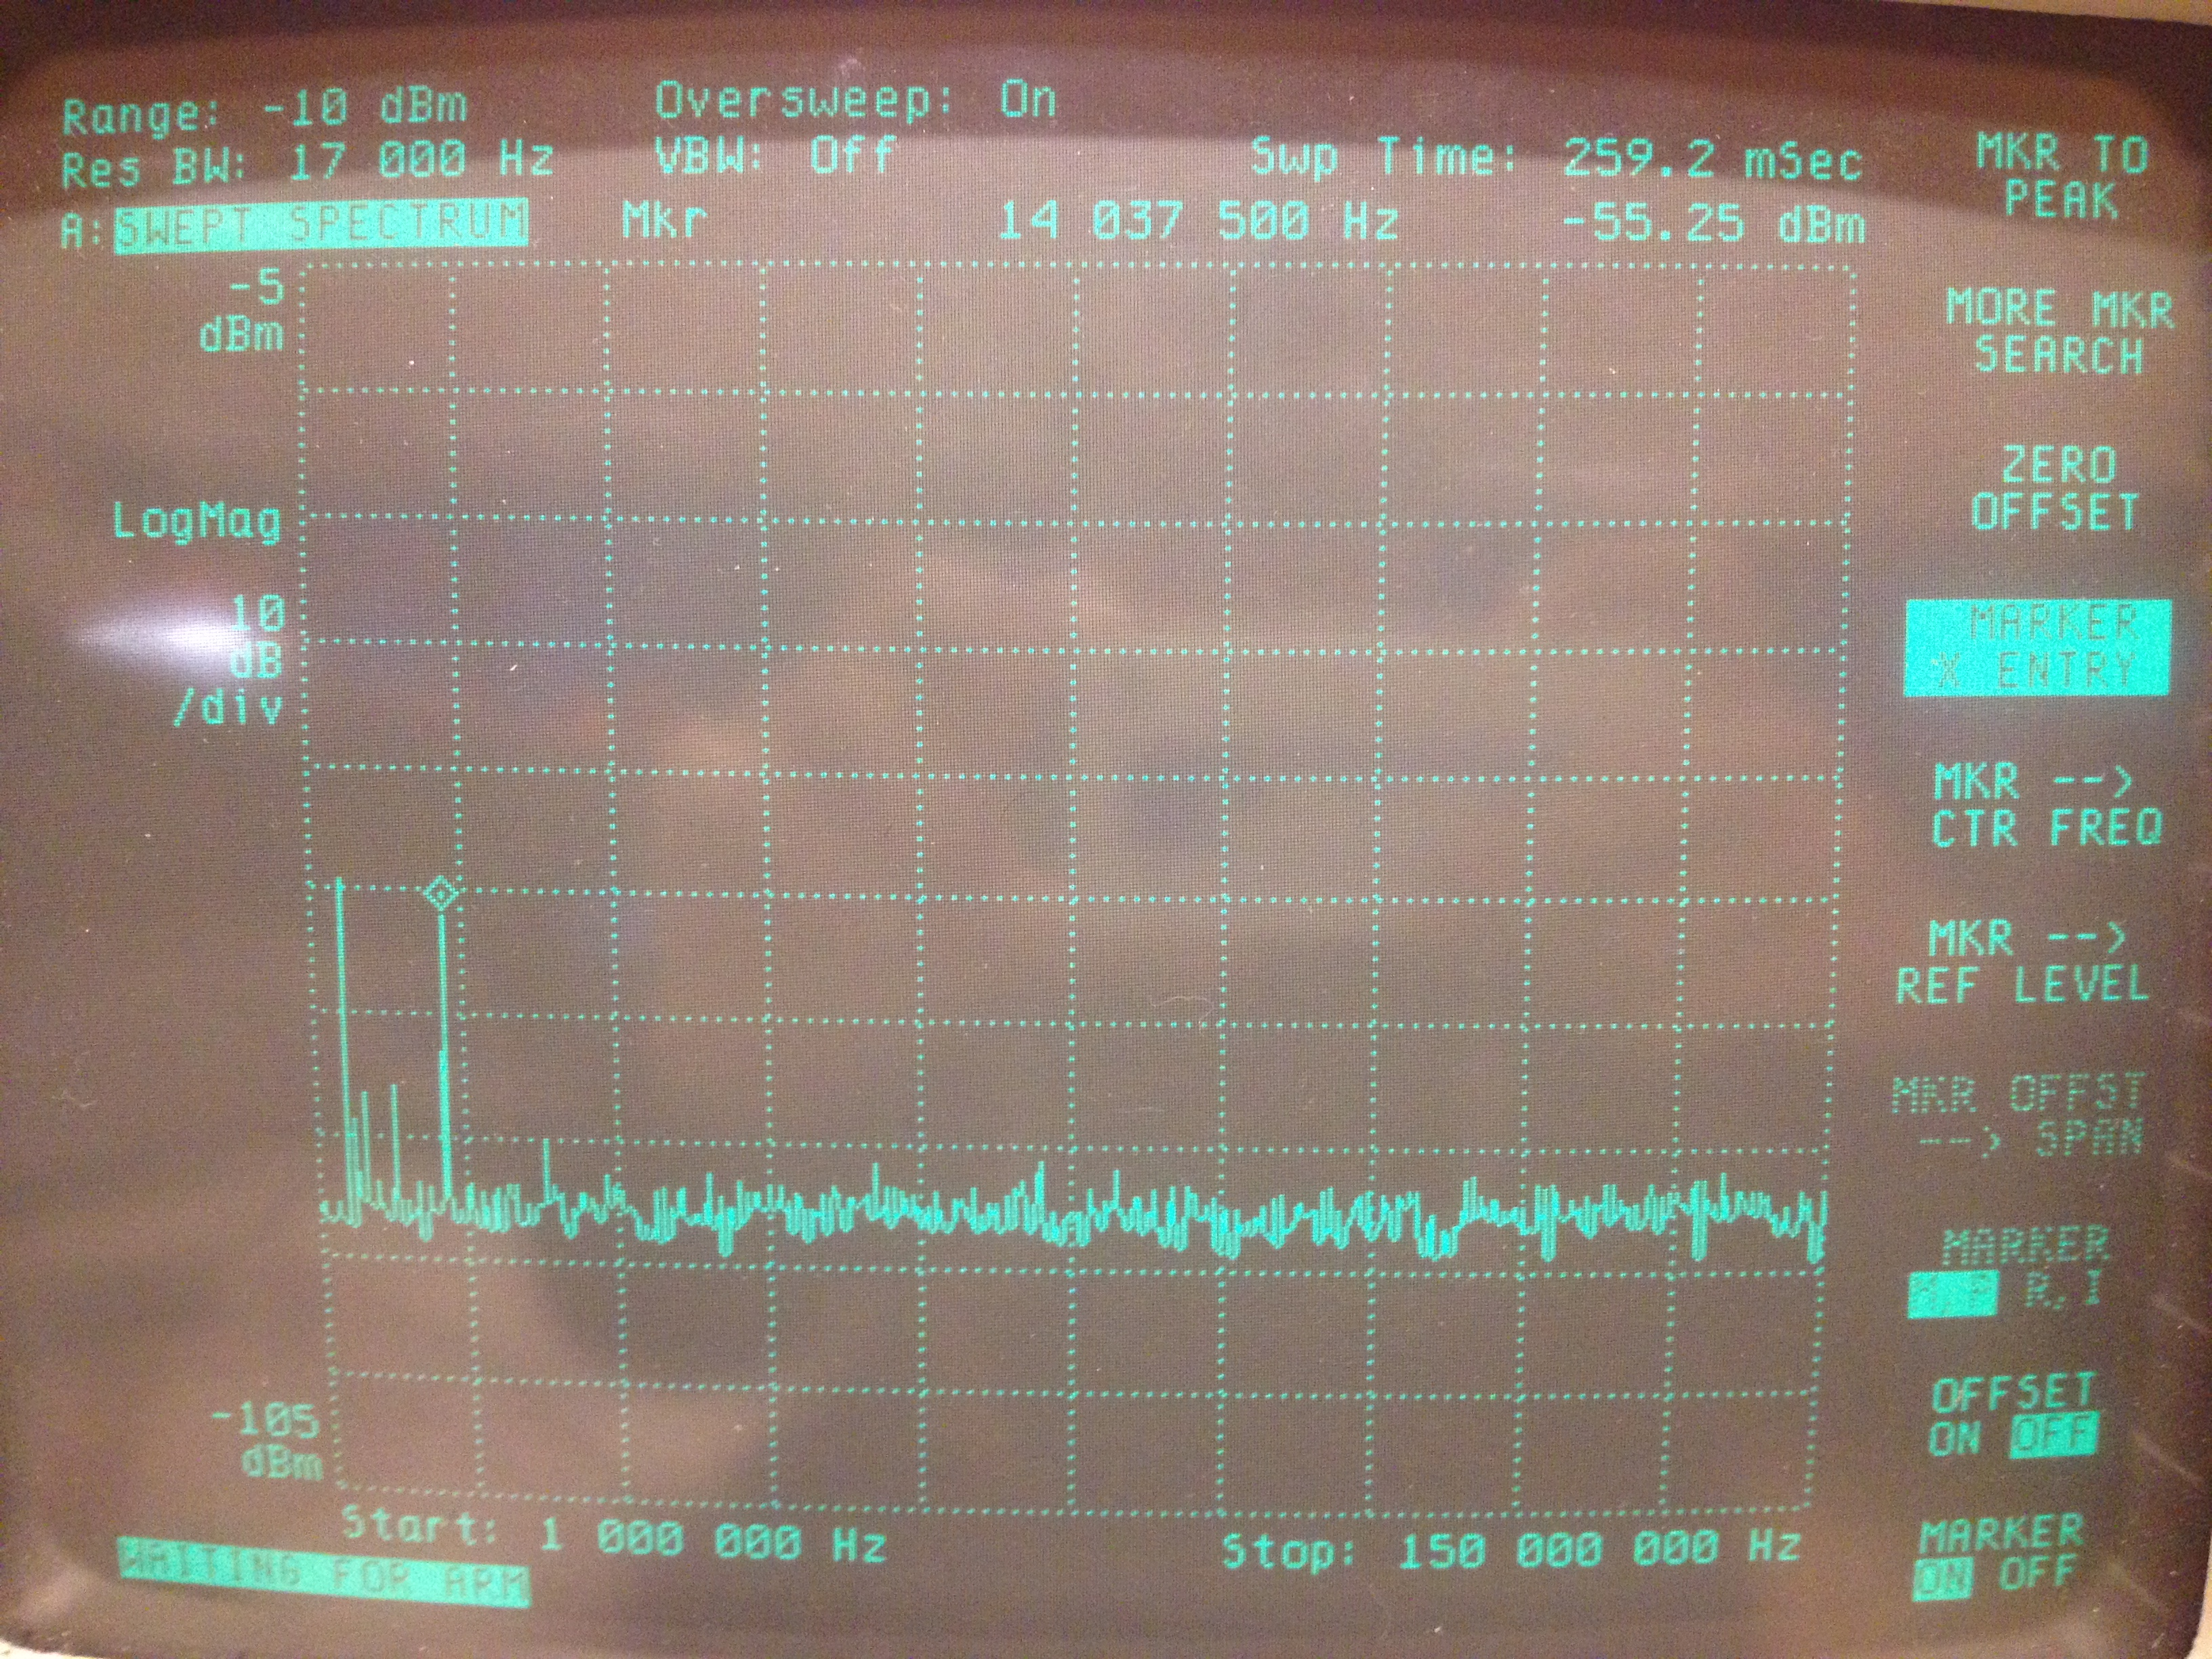
\includegraphics{8_3_1.jpg}
Mesures :
\begin{itemize}

\item Guain de conversion : 13.3 dB
\item Point de compression de 1dB : -8.2 dBm
\item Taux de distortion d'intermodulation d'ordre trois :
\end{itemize}

A noter qu'il y a une perte de puissance considérable à cause du changement d'impédance. On perd la moitié du signal d'entrée utile sur le diviseur formé par $R_{in}$ et R51, soit -6 dB. On perd une grande partie de la puissance de sortie à cause du diviseur formé par R53 et R54, les pertes sont de :
\begin{center}
$Pertes = 20\cdot \log (\frac{R54 // R_{out}}{(R54 // R_{out})+R53}) = 20\cdot \log{25}{25+1500}) \simeq -35.7 dB$
\end{center}

%  9
%
%  In 9MHz = +7 dBm
%  In 5MHz = -7 dBm
%  Pic en sortie à 14MHz = -12.5 dBm
%  => Gain de conversion = -5.5 dB
%
%  In 5Mhz = 1 dBm  =>  Pic sortie 14MHz = -5.5 dBm, soit gain = -6.5 dBm
%  => Point de compression : In RF à 1dBm, soit 0.250 Veff
%
%  In1: 9MHz = 7 dBm
%  Out: 50.47 Ohm
%  In2: analyseur de spectre  =>  -58.5 dBm
%  =>  Gain = -67.5 dB
%


% 10
%
% On prend R77 = 560, R76 = 3.3k (on veut R76/R77=6)
% L72 pour fixer à 0 le potentiel moyen à G1 (sinon, on ne contrôle pas ce potentiel moyen). Comme ça, on peut polariser négativement blablabla G1.
%
% LO : 5MHz, 1Veff, 13.01 dBm
% RF : 9MHz, 10mVeff, -27dBm
% Sortie : plein d'harmoniques : multiples de 5MHz, de 9MHz, 9-k5 ...
% 14 MHz : -56.63 dBm
% Gain : -30.37 dB avec les réductions en entrée (Rin, R72) (-6dB) et en sortie (R73,R74,Rout) (-35.7 dB)
%    soit, sans ces adaptations : 11.33 dB
% Compression 1dB : In à -3.4 dBm, soit 0.151 Veff
%
% In2 : 5 MHz, 1 Veff
% IN1 : 9.1 MHz, 8.9 MHz, -5.4 dBm, 0.12 Veff
% => 14.3 MHz (3e harmo mesurée) : -70.9 dBm
%   (14.1 MHz : -42dBm)
%
% Avec 50.47ohm en sortie, IN2 avec 1Veff (13.01 dBm), l'analyseur sur IN1 :
% on mesure à 5MHz : -62.8 dBm
%  => -75.8 dB


% 11
%
% In1 : 10 mVeff, 9 MHz, -27 dBm
% In2 :  2 Veff,  5 Mhz, 19 dBm
% Sortie 14MHz : -80.1 dBm
% Gain : -53.1 dBm
% En prenant en compte les diviseurs de tensions internes : -11.4 dBm
% On réalise qu'en augmentant légèrement In1 à partir de 10mVeff, le gain augmente légèrement,
% avant de devenir constant pour une large gamme d'amplitudes pour In1.
% On fait donc les mesures de gain pour une amplitude de In1 légèrement supérieure à 10 mVeff :
% 20 mVeff
%
% in1 : 20 mVeff, -21 dBm
% Sortie 14MHz : -75 dbm
% Gain : -54 dBm
% En prenant en compte les diviseurs de tensions internes : -11.4 dBm
%
% In1 : 18.5 dBm  =>  Sortie 14MHz : -36.6 dBm
% = Gain de compression à -1dB
%
% In1 13.9 MHz, 14.1 MHz : 1.88 Veff, 18.5 dBM
% Sortie 14.3 MHz : -70.2 dBm
%









\end{document}